\documentclass[thesis.tex]{subfiles}
\begin{document}

\chapter{Related Work}
\section{Fourier Transform}

In mathematics the fourier transform is a function that approximates a one-dimensional signal in the time domain by a sum of sine and cosine functions with different frequencies. The result is then in the frequency domain. This means the signal is represented by frequencies, amplitudes and phases.
\\ 
It is possible to visualize how the fourier transform works: Consider going along the outline of a circle over time. While going along on the outline of the circle we construct a two-dimensional function in the following way. We use the elapsed time as the x-values of the constructed function. For the y-values of the function we use the y-values of the position on the circle outline at each timepoint. The resulting function is a sine wave as seen in \ref{fig:fourier}. There are three parameters that can be adjusted in this process: the radius of the circle, the speed at which we go along the outline of the circle, and the starting position on the outline of the circle. \\
Sine waves are defomed ny their frequency, amplitude and phase. We will now show that we can arbitrarily change the frequency, amplitude and phase of the constructed sine wave by changing the three parameters of the circle. By changing the radius of the circle we change the amplitude of the resulting sine wave. Figure \ref{fig:fourier_radius} shows that the radius corresponds to the amplitude of the resulting approximation. If we change the speed at which we go along the outline of the circle, we change the frequency of the resulting function. In figure \ref{fig:fourier_speed} we doubled the speed at which we go along the outline of the circle compared to \ref{fig:fourier}. This results in a sine wave with double the frequency. Also, by changing the starting position on the outline of the circle, we can change the phase of the sine wave.\\
So far we only constructed simple sine waves. We can also construct more complex functions by using multiple circles: Instead of going along the outline of a single circle, we place a new circle on the outline of the previous circle. Each new circle moves along the outline of the previous circle. By repeating this, we can use an arbitrary number of circles. For the y-values of the resulting function, we then only use the y-values of the positions on the outline of the last circle. In figure \ref{fig:fourier_square} a square wave is approximated by using 4 circles. 
\\
The fourier transform works by finding the values of the three parameters for each circle to optimally approximate a given one-dimensional function. In literature the circles are refered to as \textit{harmonic circles}. The fourier transform returns only two coefficients per harmonic circle, but the two coefficients can be used to compute all three parameters. In this thesis we refer to the coefficients that describe a single harmonic circle as \textit{harmonic}. 
 \\ One important property of the fourier transform is that signals can be approximated arbitrarily well by specfying the number of harmonics to use. The more harmonics are used for the approximation, the better the approximation. Many common signals can be perfectly reconstructed using the fourier transform, but some, for example the square wave that we approximated in figure \ref{fig:fourier_square}, need an infinite number of harmonics for perfect reconstruction.\\ 

\begin{figure}[h]
\centering
\includegraphics[width=\textwidth]{6sin(x)/Animation_0246.jpg}
\caption{By going along the outline of a circle it is possible to construct a sine wave.}
\label{fig:fourier}
\end{figure}

\begin{figure}[h]
\centering
\includegraphics[width=\textwidth]{3sin(x)/Animation_0246.jpg}
\caption{Changing the radius of the circle changes the amplitude of the resulting sine wave. Compared to \ref{fig:fourier} the radius of the circle was halved and is now at three.}
\label{fig:fourier_radius}
\end{figure}

\begin{figure}[h]
\centering
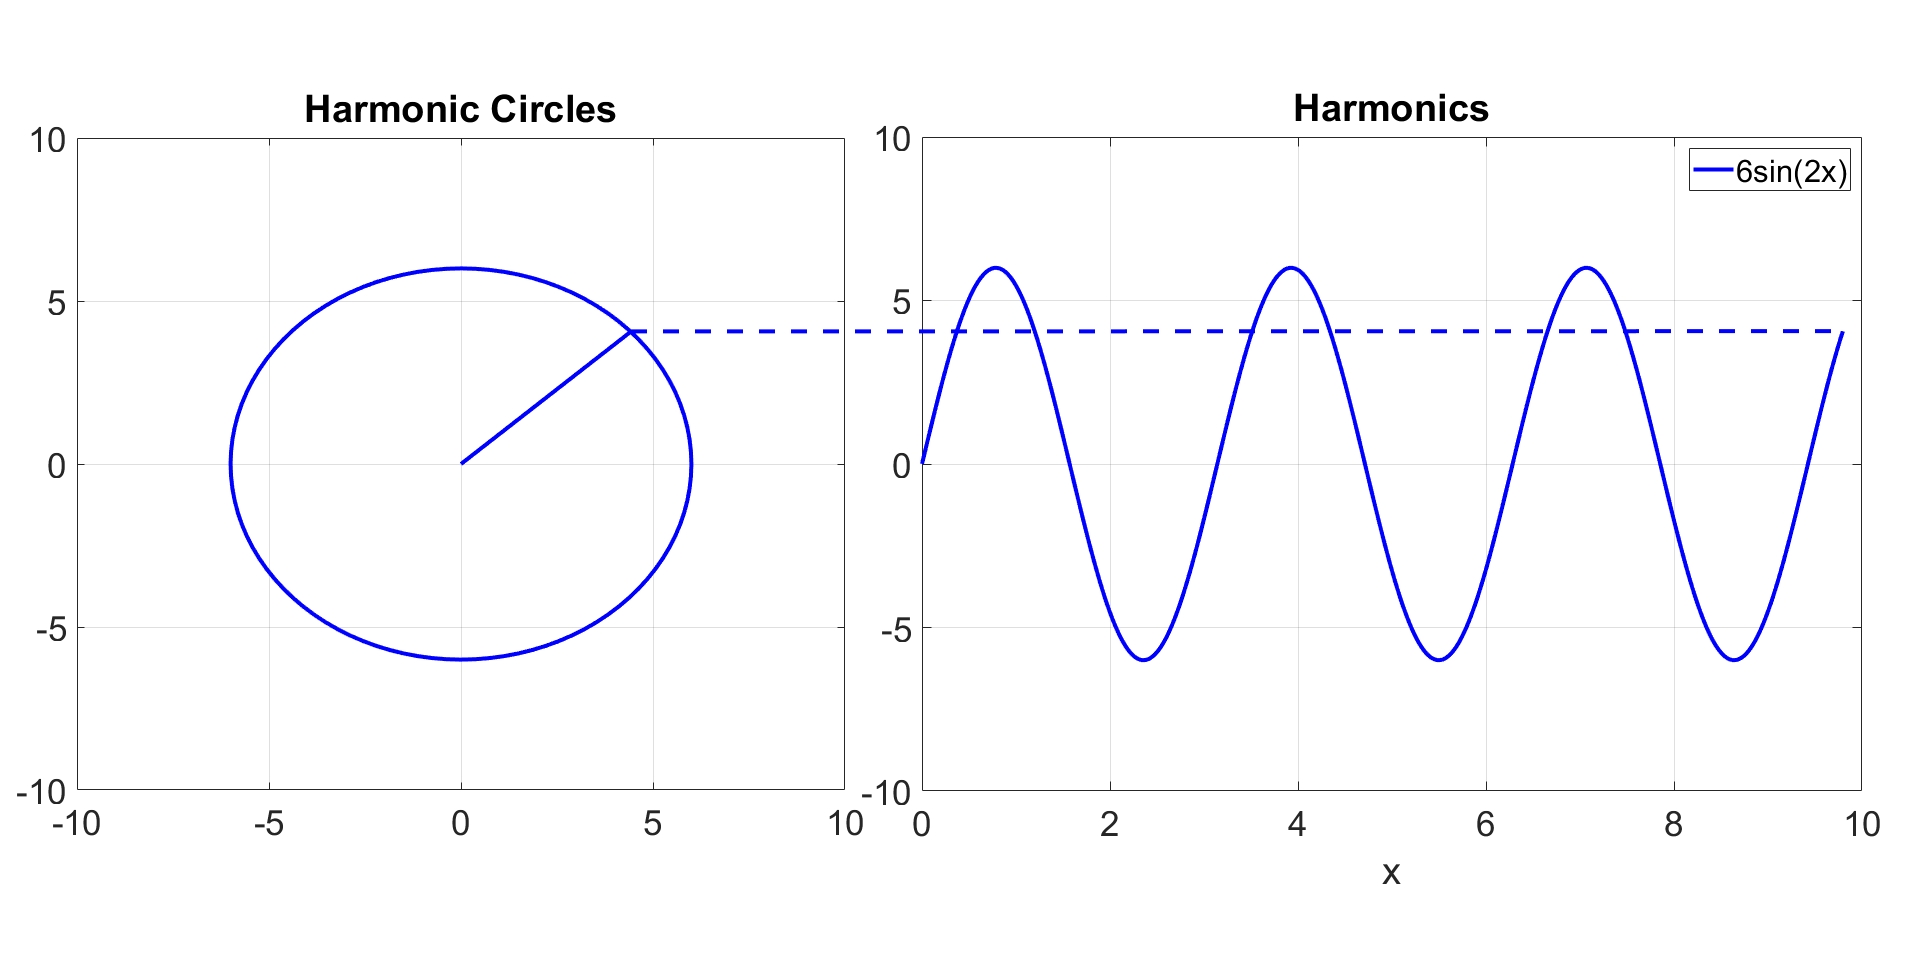
\includegraphics[width=\textwidth]{6sin(2x)/Animation_0344.jpg}
\caption{Changing the speed at which we go along the outline of the circle changes the frequency of the resulting sine wave. Compared to \ref{fig:fourier} the speed at which we go along the outline of the circle was doubled which results in a doubled frequency.}
\label{fig:fourier_speed}
\end{figure}

\begin{figure}[h]
\centering
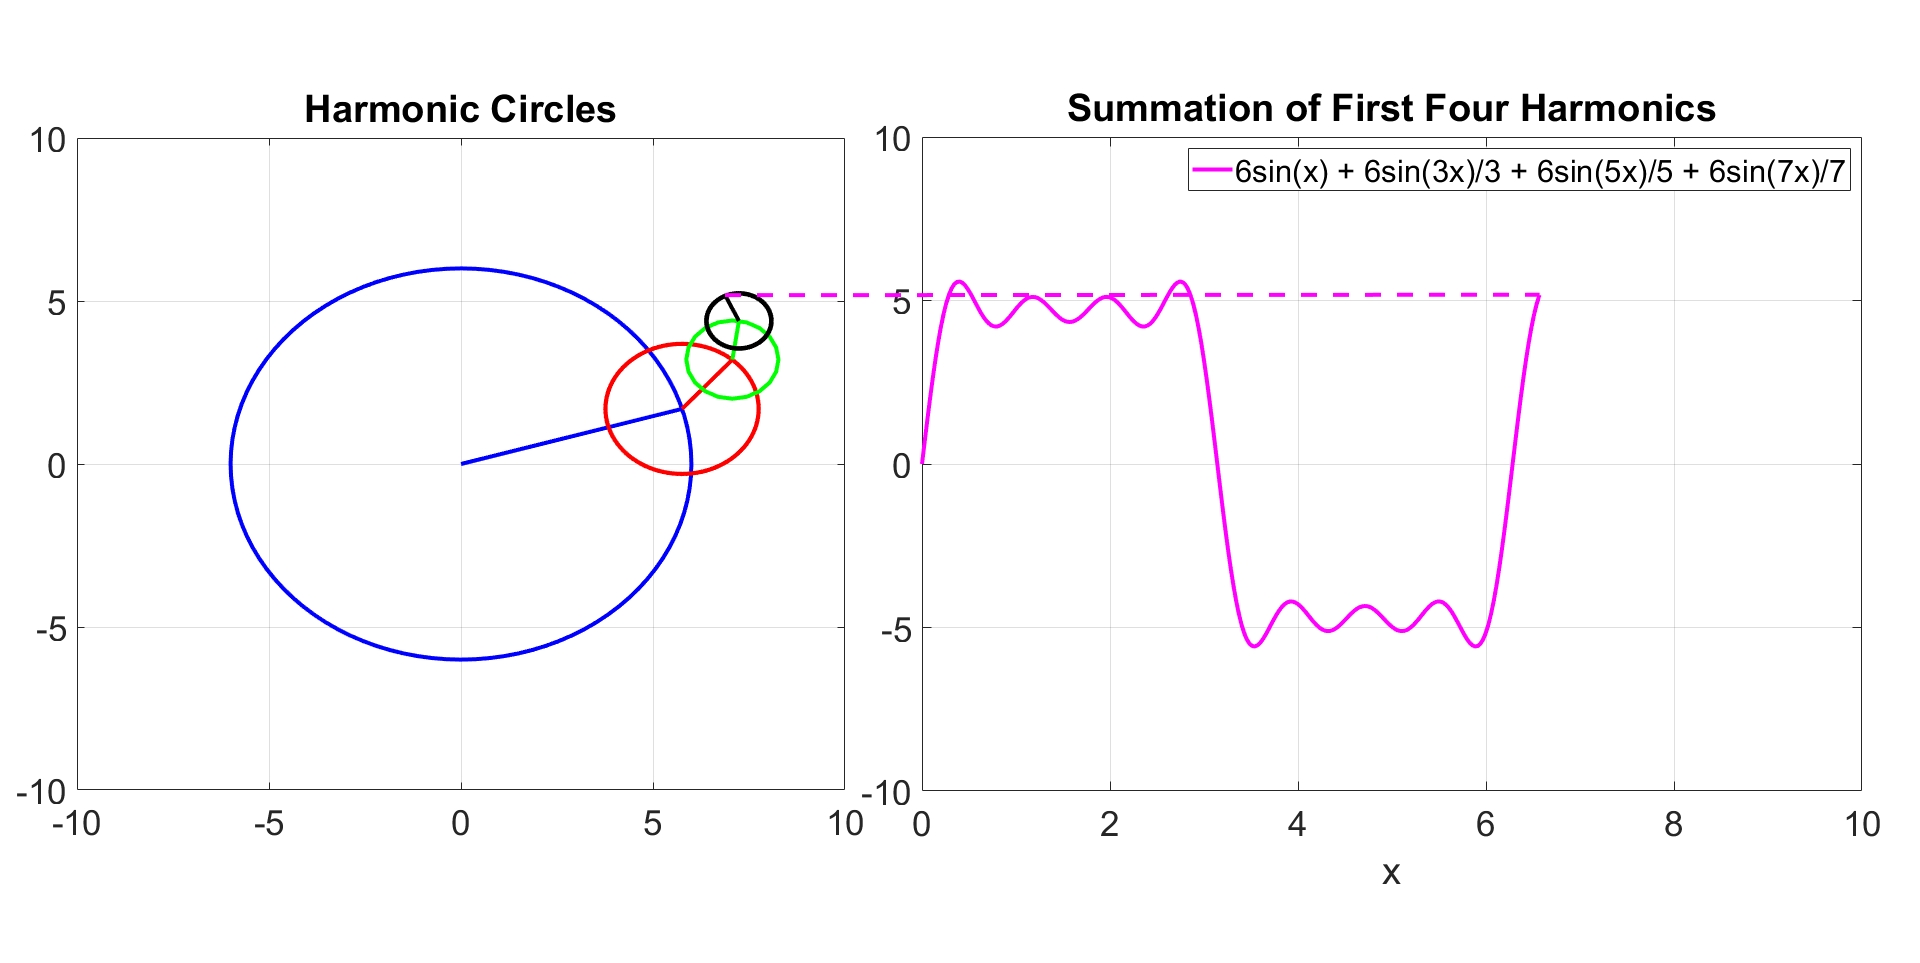
\includegraphics[width=\textwidth]{square_wave/Animation_0891.jpg}
\caption{More complex functions can be approximated by repeating the process recursively by using circles that go along the outline of the previous circle. In this case 4 circles are used to appropximate a square wave.}
\label{fig:fourier_square}
\end{figure}

\subsection{Discrete Fourier Transform}
Several different versions of the fourier transform exist to handle different kinds of input signals. In practice signals usually are finite and discrete, because memory in computers is limited and cannot store an infinite amount of values. For such input signals the \textit{Discrete Fourier Transform} (DFT) can be used. The DFT is a version of the fourier transform that can handle discrete and finite signals. Note that the DFT assumes a periodic input signal \cite{dspguide}. In our implementation we apply the fourier transform on closed contours, which are periodic, discrete, and finite. This means the DFT is suited for all input signals we use in our implementation.



%Formel und erklärung was sie macht \\
%Visualisierung \\
%Limits und probleme \\
%evntuell fehelrberechnung usw

\section{Elliptic Fourier Descriptors}
In this thesis we will use Elliptic Fourier Descriptors (EFDs) to represent the shape of the TL and FL. An EFD is a set of fourier coefficients, that can be used to reconstruct a shape. The fourier transform is only defined for one-dimensional signals, but it is possible to use it for an arbitrary number of dimensions by viewing each dimension as a separate signal. In this thesis the shapes of the lumen are defined in 2D, therefore we have to use the fourier transform twice, once for the x-direction and once for the y-direction. This means for a 2D shape we get 4 fourier coefficients per harmonic circle. The EFD of such a 2D shape contains those fourier coefficients. The first two coefficients describe the shape in x-direction and the other two coefficients describe the shape in y-direction. Combined they describe an ellipse, therefore the name Elliptic Fourier Descriptors. An important feature of EFDs is that the harmonic coefficients can be lineary interpolated to achieve a linear interpolation of the reconstructed signals. We will use this property to interpolate between shapes. 

\section{Chain Encoding Schemes} 
In this thesis we have to describe the contours of the lumen. This can be trivially done by using the pixel coordinates of the contour pixels in an ordered manner. However, there are other, often more advantageous ways to represent contours. One of them is the description of the contour by using chain codes. The Freeman Chain Encoding Scheme \cite{freeman} for example encodes the contour by using number from 0 to 7. For each pixel the number describes the direction to the next pixel relatively to the the current pixel. The numbers used for each direction are shown in figure \ref{fig:freeman}. An example is the triangle shown in figure \ref{fig:pixel_triangle} that can be described by the freeman chain code 111777444444 \\  
One advantage is that a contour described by a freeman chain code is invariant to translations. Another advantage is that different freeman chain codes can be directly compared, as long as the same starting pixel was used. Freeman Chain Codes are not invariant to the picking of the starting pixel, but they can be normalized to be: Picking of a different starting pixel when creating the freeman chain code results in a circular shift of the chain code. To obtain a chain code that is invariant to picking of different starting pixels we can circularly shift the chain code until we find the chain code that produces the lowest possible number \cite{Ballard:1982:CV:578131}. \\  Freeman chain codes are not invariant to rotations. A way to (partially) make them invariant to rotations is to store the differences of the chain code segments instead of storing the directions from one pixel to the next. Computationally this can be done by subtracting each chain code segment from the next and taking the result modulo $n$, where $n$ is the connectivity. The freeman chain code is 8-connected, therefore we set $n = 8$. In literature such chain codes are called \textit{differential chain codes}. As an example, if we use the freeman chain code of the triangle in figure \ref{fig:pixel_triangle}, then the resulting differential chain code is 00600300000.  \\
An different chain code encoding scheme is the vertex chain code (VCC) \cite{vertex_chain_code}. The VCC does not follow the pixels as the freeman chain code. Instead, it follows the vertices that lie on the border between the pixels and the background. This difference becomes more apparent if we consider the chain codes of a single pixel. In such a case the freeman chain code consists of 0 elements. The VCC in this case is 1111. This is because the VCC moves along the 4 edges of the pixel. Each segment of the VCC indicates the number of cell vertices, which are in touch with the bounding contour of the shape at that position. The VCC can be used for rectangular (pixels), triangle or hexagonal cells. In the following we will describe the reconstruction only for the case of rectangular cells, as that case is the only one that is relevant in this thesis. In the case of rectangular cells the element values range from 1 to 3. \\ To reconstruct the contour from a chain code several steps have to be done: First each element of the VCC is converted to a \textit{slope change} as defined by the slope change notation in \cite{slope_change_notation}. In the case of rectangular cells this specifically means that the element values 1, 2 and 3 are replaced by 0.5, 0.0, and -0.5 respectively. Then the integral of this slope change chain code is computed, which is the addition of the elements, element by element. For example consider the slope change chain code 1.0 0.5 0.0 -0.5. The first element of the integral is then 1.0. The second element is 1.5 (1.0 + 0.5). The third element is 1.5 (1.0 + 0.5 + 0.0) and the last element is 1.0 (1.0 + 0.5 + 0.0 - 0.5). The finished integral is then 1.0 1.5 1.5 1.0. Each element of the integral can be used to compute the x- and y-displacement from one vertex to the next using the equations in \ref{eq:vcc_reconstruction}. $C_{x_i}$ and $C_{y_i}$ are the displacements described by the $i$-th element in the integral in x- and y-direction respectively. $l$ is the length of one side of a cell. $c_i$ is the current element of the integral. 

\begin{equation} \label{eq:vcc_reconstruction}
\begin{split} 
C_{x_i} = l  cos(\pi c_i) \\
C_{y_i} = l  sin(\pi c_i) \\
\end{split}
\end{equation}

\begin{figure}[h]
\centering
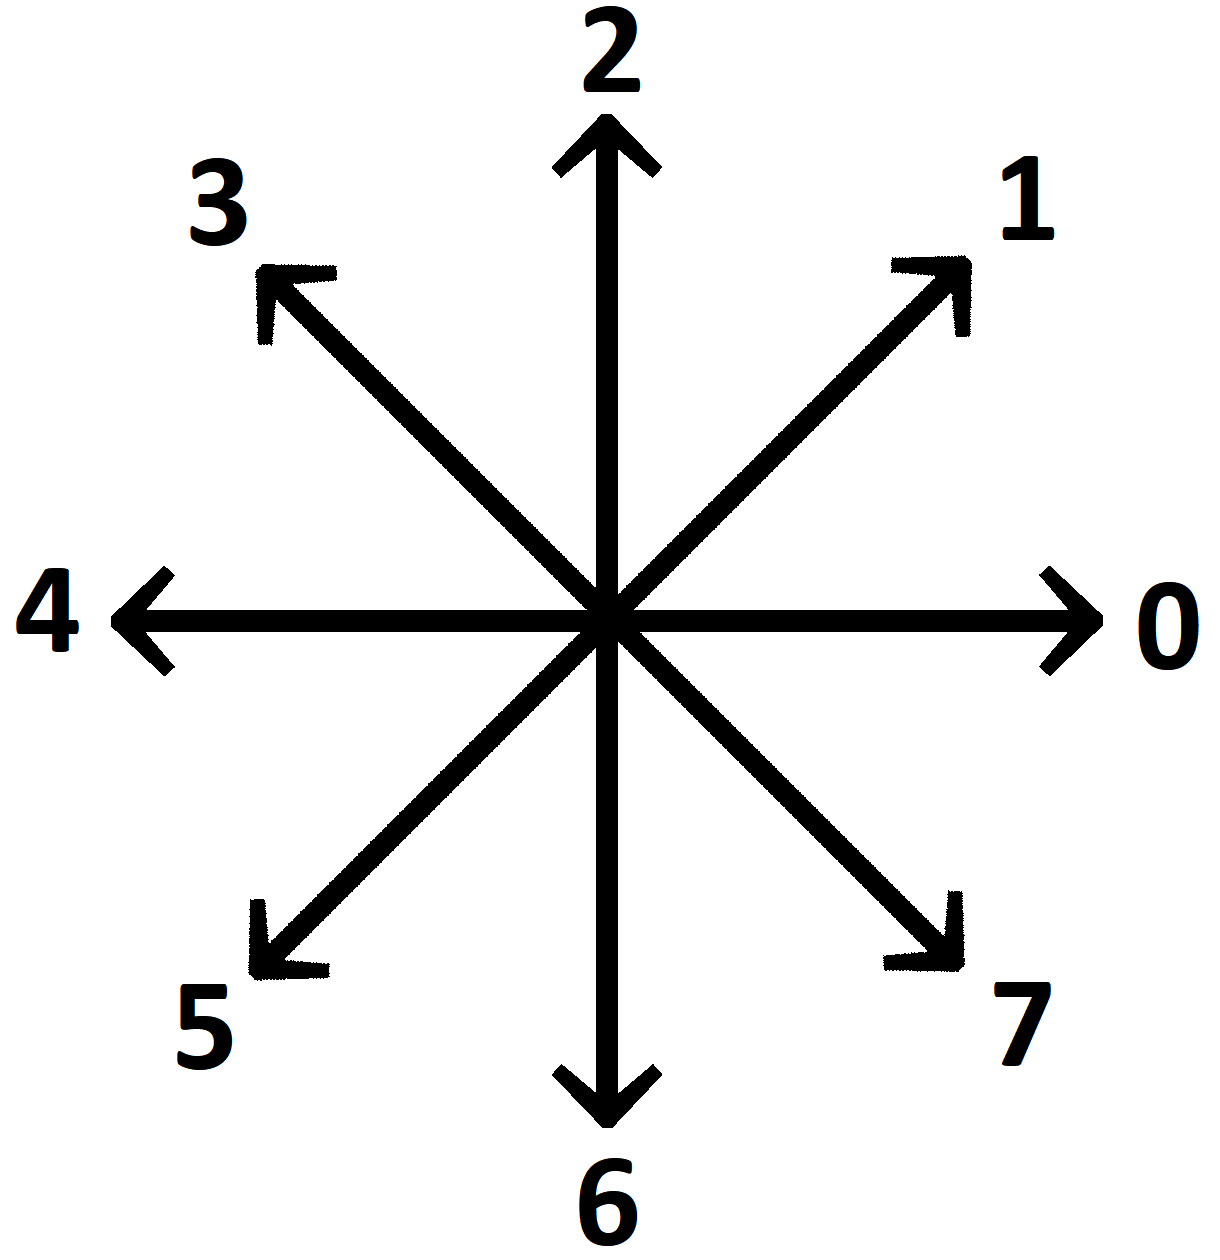
\includegraphics[width=\textwidth/3]{chaincode.png}
\caption{The numbers of the freeman chain code. The next pixel is described by a number of 0 to 7 depending on where it is located in the 8-neighborhood of the current pixel.}
\label{fig:freeman}
\end{figure}

\begin{figure}[h]
\centering
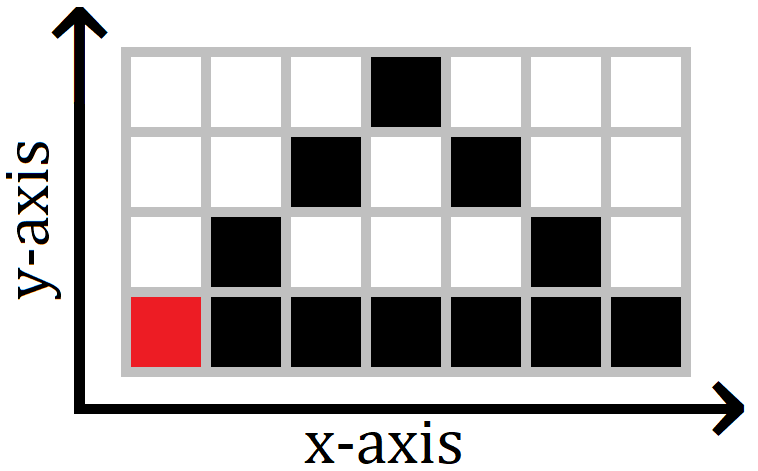
\includegraphics[width=\textwidth/2]{pixel_triangle.png}
\caption{A triangle composed of pixels on a grid. The red pixel is the startng pixel. A possible freeman chain code of this triangle is then 111777444444. The differential chain code of this freeman chain code is 00600300000.}
\label{fig:pixel_triangle}
\end{figure}

\subfilebib % Makes bibliography available when compiling as subfile
\end{document}